\section{Key Requirements}
\subsection{Terms, definitions and abbreviated terms}
\subsubsection{Terms and Definitions}
\begin{itemize}
    \item \textbf{OAuth}: Authentication protocol that allows one application 
    to interact with another one on behave of the first one.
    \item \textbf{Firebase Cloud Messaging}: Cross-platform message and 
    notification solution develop by Google.
    \item \textbf{Customer}: User who is going to search products and create 
    order by purchasing products from merchants.
    \item \textbf{Merchant}: User that upload products to the store, 
    inside the platform, from which the customers are going to purchase. 
    \item \textbf{Driver}: User that fulfills the order generated by the 
    customer. 
    \item \textbf{Order}: A list of items that were paid by a customer and 
    is going to be fulfilled by a driver.
    \item \textbf{Cart}: Container that holds, temporarily, a group of products 
    that are going to be purchased.
    \item \textbf{Estimated time of Arrival}: The amount of time that 
    an order is going to take before arriving to the customer.
    \item \textbf{Interaction}: Amount of touches required by the user to 
    perform an action, if the device has a touch screen, or the amount of 
    clicks a user performs, if the device has a non-touch screen.
    \item \textbf{2FA}: Authentication method in which a particular device is 
    used to grand access to a website or application, this method requires 
    two or more pieces of evidence that confirms the user identity.
    \item \textbf{JWT}: An open standard method for representing claims 
    securely between two parties.
    \item \textbf{PCI}: set of security standards designed to ensure that ALL 
    companies that accept, process, store or transmit credit card 
    information maintain a secure environment. \cite{pci}
\end{itemize}
\subsubsection{Abbreviated Terms}
\begin{center}
    \begin{tabular}{p{0.40\textwidth}p{0.60\textwidth}}
    \hline
    \textbf{Abbreviation} & \textbf{Term} \\ 
     \hline
     PSS & Personal Shopper System \\  
     \hline
     PSMS &  Personal Shopper Merchant System \\  
     \hline
     PSDS &  Personal Shopper Driver System \\  
     \hline
     PSSS &  Personal Shopper Server System \\  
     \hline
     FCM &  Firebase Cloud Messaging \\  
     \hline
     ETA & Estimated time of Arrival \\  
     \hline
     2FA & 2-Factor Authentication  \\  
     \hline
     JWT & JSON Web Token  \\  
     \hline
     JSON & JavaScript Object Notation \\ 
     \hline
     PCI & Payment Card Industry \\ 
     \hline
     VM & Virtual Machine \\ 
     \hline
     AWS & Amazon Web Services \\ 
     \hline
     CI & Continuous Integration \\ 
     \hline
    \end{tabular}
\end{center}
\pagebreak
\subsection{Assumptions and Dependencies}
\begin{enumerate}[label=AS-\arabic*]
    \item The market share that the application is going after, is the online 
    shopping market where the store and the merchants exist near to each other.
    \item We will use the HEART model \cite{heart} to measure improvements 
    in UI/UX designs.
    \item Drivers already sign up in the system when they send their 
    driver application to the company, outside of the project scope.
    \item Merchants are already added into the system, outside of the 
    project scope.
    \item There is only one account per merchant. \textit{At least in the first 
    iteration.}
    \item The merchants are going to submit products that are appropriate for 
    all ages. \textit{They are not going to upload drugs, guns, medical 
    devices}.
    \item The merchants are already sign a contract that specify the types of 
    products they can add in the platform.
    \item Customers have 2FA \cite{2fa} as an option.
    \item Merchants require 2FA.
    \item Drivers have 2FA as an option.
    \item A driver session, for a specific driver, can only run on one 
    device at a time.
    \item PSS, PSMS, PSDS only talk with PSSS, using a request-response 
    approach.
    \item Installing PSSS requires that a trained operator perform 
    the installation.
    \item Android is the only mobile platform. iOS is going to be target in 
    future releases.
    \item The customer order would be sent to the nearest driver to the 
    merchant store.
    \item A \textbf{disabled} product, is a product that do not get displayed 
    in PSS.
    \item Opening and closing times for merchants are going to be set outside 
    of the scope of the project.
\end{enumerate}
\begin{figure}[!htb]
    \centering
    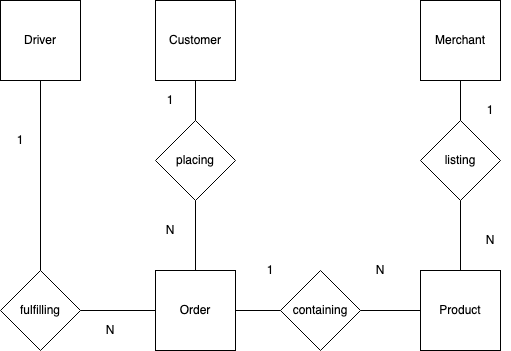
\includegraphics[scale=0.50]{Logical Data Model.png}
    \caption{Logical Data Model}
\end{figure}

\begin{enumerate}[resume, label=AS-\arabic*]
    \item Merchants are small businesses that usually have no more 
    than 5 employees in a single shift.
    \item All the merchants, customers and drivers operate inside the 
    Hoboken area.
    \pagebreak
    \item PSS have two versions mobile which is Android and a Web version.
    \item PSMS has only a web version.
    \item PSDS has only an Android version.
    \item PSSS is an API server only.
    \item Notifications in PSS (Mobile/Web) and PSDS are going to use FCM.
\end{enumerate}
\pagebreak
\subsection{Business/Mission Requirements}
\begin{enumerate}[label=BR-\arabic*]
    \item As a platform, we want to increase transactions to 15 a day for each 
    merchant within the first 6 months since the launch date.
    \item Keep customer satisfaction as high as posible, a 9 out of a 10 scale 
    within the first 6 month of release.
    \item Achieve the break-even point in 6 months.
    \item Increase transactions to at least 50 a day, by merchant, within 
    a year.
    \item Achieve positive cash flow on this product within a year.
    \item Increase market share in Hoboken to 2\% within a year.
    \item Increase market share in Hoboken to 4\% in the second year.
    \item Reduce delivery time by 5\% in the first 6 months.
    \item Reduce delivery time by 10\% in the first year.
    \item Comply with federal laws and regulations.
    \item Achieve product market fit \cite{product-market-fit} within the first 
    year from release.
    \item Become the application with the biggest amount of stores partnered 
    with our services in Hoboken within the first year.
    \item Be the application with the largest amount drivers in Hoboken 
    within the first two years.
    \item Increase the amount of stores affiliated to the application to 12 
    stores after 3 months from release.
    \item Increase the amount of stores affiliated to the application to 30 
    stores after 6 months from release.
    \item Increase the amount of stores affiliated to the application to 100 
    stores after 12 months from release.
    \item Increase the amount of stores affiliated to the application to 150 
    stores after 18 months from release.
    \item Expand to nearby cities within the first three years since release
    \item Increase the amount of drivers enrollment to 50, within the first 
    6 months since release.
    \item Increase the amount of drivers enrollment to 100, within the first 
    2 months since release.
    \pagebreak
    \item Increase the amount of drivers enrollment to 150, within the first 
    24 months since release.
    \item Increase merchant sales by 20\% within the first 24 months of launch.
    \item Achieve 30, 000 USD in gross profit at the end of the first year
    \item Increase the amount of employees by 2 in the first two years
    \item Increase company gross margin at a rate of 10\% from the previous 
    year, each year.
    \item Improve UI/UX in our products between the first and second year 
    since launch. \textit{We will improve it by iterating periodically. See 
    requirement AS-2}.
    \item Reduce monthly support cost by 10\% after the first year. 
    \textit{This refers to the customer support provided to support inquiries 
    coming from merchants, drivers or customer of the platform, this customer 
    support is outside of the scope of the project.} 
\end{enumerate}
\pagebreak 
\subsection{User Requirements}
\subsubsection{Merchants}
\begin{enumerate}[label=USR-\arabic*]
    \item As a merchant i want to authenticate in the application.
    \item As a merchant i want to be able to update my password.
    \item As a customer i want to be able to logout.
    \item As a merchant i want to add products into the application.
    \item As a merchant i want to set the prices to the products.
    \item As a merchant i want to disable existing products.
    \item As a merchant i want to update existing products.
    \item As a merchant i want to remove existing products.
    \item As a merchant i want to re-enable products that are disabled.
    \item As a merchant i want to group products in categories.
    \textit{Categories are a way to group products that shared a particular 
    characteristic, a product can only belong to one category at a time}.
    \item As a merchant i want to set possible substitution for related items.
    \item As a merchant i want to group products in different type of 
    collections. \textit{Collection is a way to group products arbitrarily 
    (Sales, Promotions, Seasons), a product can belong to one or more 
    collections.}
    \item As a merchant i want to be able to reach out for technical support.
\end{enumerate}
\subsubsection{Customers}
\begin{enumerate}[resume, label=USR-\arabic*]
    \item As a customer i want to authenticate in the application.
    \item As a customer i want to be able to update my password.
    \item As a customer i want to be able to logout.
    \item As a customer i want to see the available merchants near me.
    \item As a customer i want to see the available products from a single 
    merchant.
    \item As a customer i want to see where are the merchants in a map.
    \item As a customer i want to see where i’m in a map.
    \item As a customer i want to be able to add my credit card information 
    to my profile.
    \item As a customer i want to upload my photo to my profile.
    \item As a customer i want to save my favorite merchants.
    \item As a customer i want to be able to see the information of the driver 
    that is bringing the order.
    \item As a customer i want to know what is the ETA for the order to arrive.
    \item As a customer i want to know when the driver is on their way to the 
    merchant store.
    \item As a customer i want to know when the driver is working on the order.
    \item As a customer i want know when the driver is on their way to deliver 
    the order.
    \item As a customer i want to able to rate the driver.
    \item As a customer i want to be able to tip my driver.
    \item As a customer i want to be able to cancel an order.
    \item As a customer i want to be able to set replacements in case a 
    product is not found.
    \item As a customer i want to see all the products in a category, from a 
    merchant page.
    \item As a customer i want to see all the collections from a merchant.
    \item As a customer i want to be able to message a driver.
    \item As a customer i want to know the contact information of a 
    particular merchant.
    \item As a customer i want to be able to reach out for technical support.
    \item As a customer i want to be able to search a product 
    \item As a customer i want to be able to sort products by price 
    \item As a customer i want to be able to sort merchants by distance 
\end{enumerate}
\pagebreak
\subsubsection{Drivers}
\begin{enumerate}[resume, label=USR-\arabic*]
    \item As a driver i need to authenticate in the application
    \item As a driver i want to be able to update my password
    \item As a driver i want to be able to sign out
    \item As a driver i need to notify the system that i am ready to 
    accept orders
    \item As a driver i need to accept orders
    \item As a driver i need to deny orders
    \item As a driver i need to delivered orders to an address
    \item As a driver i need to notify the customer that i’m on my way to the 
    merchant store
    \item As a driver i need to notify the customer that i’m working on the 
    order
    \item As a driver i need to notify the customer that i’m on the way to 
    deliver the order
    \item As a driver i need to be able to message a customer in case an 
    item is not available
    \item As a driver i need to see a history of all the orders i delivered
    \item As a driver i need to be able to take a picture, when the order is 
    delivered
    \item As a driver i want to know if i am in an available area to receive 
    orders
    \item As a driver i want to know the route to deliver the customer order
    \item As a driver i want to be able to see the items in the order i 
    accepted
    \item As a driver i want to know the route to the merchant store from an 
    order that i accepted
    \item As a driver i want to be able to reach out for technical support
    \item As a driver i want to know how much profit i made from an order
\end{enumerate}
\pagebreak
\subsection{Operating Environment}
\begin{enumerate}[label=OE-\arabic*]
    \item The PSSS is going to run on AWS infrastructure.
    \item Image assets are going to be stored in AWS S3.
    \item New servers are going to be spin up on demand using EC2 VMS.
    \item The PSSS can only be accessed by PSS, PSMS, PSDS.
    \item Network requests coming from outside of US are going to be ignored.
\end{enumerate}
\begin{figure}[!htb]
    \centering
    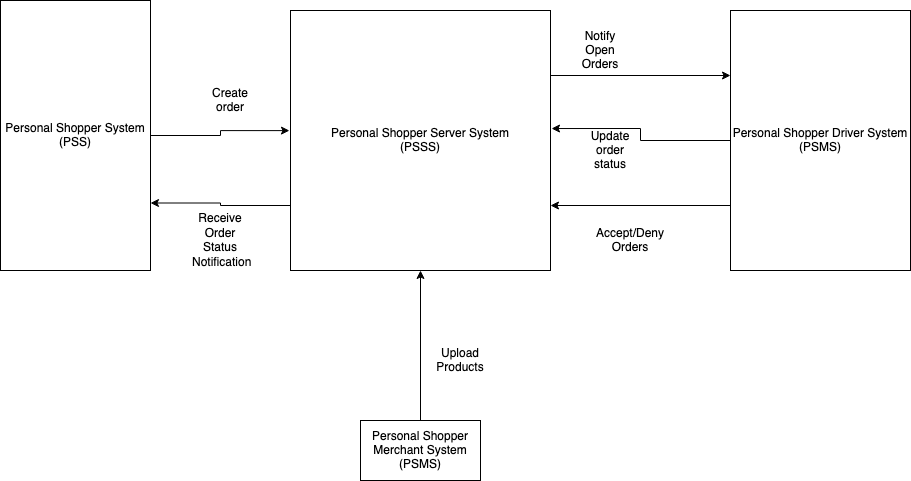
\includegraphics[scale=0.38]{Context Diagram.png}
    \caption{Context Diagram}
\end{figure}
\pagebreak
\subsection{System Requirements}
\subsubsection{General}
System refers to all the user facing systems (PSS, PSMS, PSDS)
\begin{enumerate}[label=SY-\arabic*]
    \item The system shall enable users to login into the platform.
    \begin{enumerate}[label=SY-1.\arabic*]
        \item The system shall request the user to input the following required 
        fields:
        \begin{itemize}
            \item Email
            \item Password
        \end{itemize}
        \item The system shall display an error message if the one of the fields 
        to be entered is empty.
        \item The system shall display an error message if formatting for one 
        of the fields is incorrect.
        \item The system shall display an error message if the email and 
        password do not matched the previsouly store credential.
    \end{enumerate}
    \item The system shall enable users to close current session.
    \item The system shall enable users to update their passwords.
\end{enumerate}
\subsubsection{Personal Shopper System}
\begin{enumerate}[resume, label=SY-\arabic*]
    \item PSS shall enable a customers to sign up:
    \begin{enumerate}[label=SY-4.\arabic*]
        \item PSS shall request that customer fill their information by
        writing inside input text requesting the following fields:
        \begin{itemize}
            \item Name
            \item Last name
            \item Phone number
            \item Email
            \item Password
            \item Confirm Password
        \end{itemize}
        \item PSS shall display an error message if one of the fields is empty.
        \item PSS shall display an error message if the format is incorrect.
        \item PSS shall display an error message if the passwords do not match.
    \end{enumerate}
    \item PSS shall enable customers to signup into the platform by using an 
    authorized public OAuth implementation:
    \begin{itemize}
        \item Google Sign-in \cite{google-sign-in}
        \item Sign in with Apple \cite{sign-in-with-apple}
    \end{itemize}
    \item PSS shall display a message that suggest the user to sign up in
    response to a failed login in case the email address that they 
    insert does not exist in the platform
    \item The PSS shall enable customers to login into the platform by using 
    authorized public OAuth implementation:
    \begin{itemize}
        \item Google Sign-in \cite{google-sign-in}
        \item Sign in with Apple \cite{sign-in-with-apple}
    \end{itemize}
    \item PSS shall display a list of all the available merchants.
    \begin{enumerate}[label=SY-8.\arabic*]
        \item PSS shall use the device GPS to locate registered merchants that 
        are in a 2 mile radius from the customer position.
        \item If no merchants are found, it displays the message "No merchants 
        are in your area".
        \item PSS shall display the merchants as 
        cards. \cite{material-design-cards}
        \item PSS shall display merchant information: 
        \begin{itemize}
            \item Name
            \item Address
            \item Image
            \item Phone
            \item Distance between the customer and the merchant, in meters.
        \end{itemize}
    \end{enumerate}
    \item PSS shall display what is the customer current location 
    inside a map.
    \item When the customer is inside a merchant page, PSS shall enable the 
    customer to search a product.
    \begin{enumerate}[label=SY-10.\arabic*]
        \item PSS shall show a list of products, that matches the search, 
        and display the following fields.
        \begin{itemize}
            \item Product name
            \item Image 
            \item Short description
            \item Price
        \end{itemize}
    \end{enumerate}
    \end{enumerate}
    \begin{enumerate}[resume, label=SY-\arabic*]
    \item PSS shall enable customers to add a product to the cart.
    \item PSS shall enable customers to add their payment information 
    into the platform.
    \item When the cart has one or more items, PSS shall permit the user to 
    create an order.
    \item PSS shall permit customer to cancel an order.
    \item PSS shall permit customer to confirm that they received an order.
    \item If the customer forgets its password, PSS shall request to user to 
    enter its email address and shall an email with a temporary password.
    \item If there is an issue with an order, PSS shall enable customers to 
    open an ticket about the order.
    \item PSS shall enable user to send a message to the driver.
    \item PSS shall display drivers information:
    \begin{itemize}
        \item Phone Number
        \item Name
        \item Profile Picture
    \end{itemize}
    \item PSS shall display the ETA from a pending order.
    \begin{enumerate}[label=SY-20.\arabic*]
        \item PSS shall display the ETA in terms of minutes.
    \end{enumerate}
    \item PSS shall display merchants information.
    \begin{itemize}
        \item Name
        \item Phone 
        \item Email 
        \item Address
    \end{itemize}
\end{enumerate}

\subsubsection{Personal Shopper Merchant}
\begin{enumerate}[resume, label=SY-\arabic*]
    \item PSMS shall enable merchants to add a product, by requesting the 
    following required fields.
    \begin{itemize}
        \item Name
        \item Description
        \item Picture
        \item Weight
        \item Price 
        \item Tags
    \end{itemize}
    \item PSMS shall enable merchants to update a selected product.
    \item PSMS shall enable merchants to delete a selected product.
    \begin{enumerate}[label=SY-24.\arabic*]
        \item PSMS shall display a message dialog that request a confirmation 
        from the merchant.
    \end{enumerate}
    \item PSMS shall enable merchants to disable a selected product.
    \item PSMS shall enable merchant to enable products that were 
    previously disabled.
    \item If the merchant forgets its password, PSMS shall request to user 
    to enter its email address and PSMS shall send an email with a 
    temporary password.
\end{enumerate}

\pagebreak

\subsubsection{Personal Shopper Driver}
\begin{enumerate}[resume, label=SY-\arabic*]
    \item  If the driver forgets its password, PSDS shall request to user to 
    enter its email address and shall an email with a temporary password.
    \item  If the driver receives an order requests, PSDS shall request the 
    driver to accept the order.
    \item  If the driver receives an order requests, PSDS shall request the 
    driver to decline the order.
    \item  If the driver fulfills the order, PSDS shall enable the driver to 
    mark the order as delivered.
	\item  If the driver mark an order as delivered, PSDS shall request the 
    driver to take a picture of the delivery.
    \item  PSDS shall enable the driver to send a signal to PSSS that notifies 
    to the customer that the driver it's on its way to the merchant.
    \item  PSDS shall enable the driver to send a signal to PSSS that notifies 
    to the customer that the driver it's at the merchant and it's working 
    in the order.
    \item  PSDS shall enable the driver to send a signal to PSSS that notifies 
    the customer that the driver it's on its way to the deliver the order to 
    the customer.
    \item  If the driver requires to reach out to the customer, PSDS shall 
    display the phone number of the customer.
    \item  PSDS shall display a list of all the orders that the drivers 
    performer in the last 30 days.
    \item  PSDS shall display what is the driver current location inside a map.
    \item  If the driver requires technical support, PSDS shall display a 
    technical support phone number.
\end{enumerate}

\begin{figure}[htpb]
    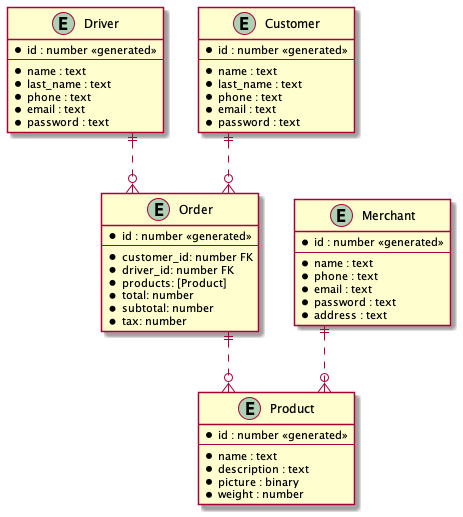
\includegraphics[scale=0.70]{data-model-diagram.png}
    \caption{Data Model Diagram}
\end{figure}
\FloatBarrier
\pagebreak
\subsection{Security Requirements}
\begin{enumerate}[label=SEC-\arabic*]
    \item The PSS shall require an email and password access to log in.
    \item PSS password must be no shorter than 8 characters, it requires
    1 special character, and 2 numbers. \textit{Special character are 
    any character under UTF-8, that is not an alphanumeric character}.
    \item The PSS shall not store passwords in plain text, it shall salt the 
    passwords and encrypt using SHA-2 algorithm.
    \item The PSS shall display an error message in the case of a failure in a 
    transaction in order to protect customer data.
    \item The PSS shall allow customers to file any reports with their orders 
    by sending an email to the support email address with the order number and 
    issue details.
    \item The PSS shall ask the customer whether or not their order has arrived 
    if it is 1 hour after the driver, gets to the store.
    \item The PSS shall allow users to delete their own account, this is also 
    shared with the PSMS and the PSDS.
    \item The PSS shall allow users to disable their own accounts for a certain 
    period of time up to 1 year.
    \item The PSS shall not store any credit card information, it will use an 
    authorized, PCI Compliant, provider to store the information. (PayPal).
    \item The PSS shall ignore all network request that comes outside of US.
    \item The PSSS shall log all information regarding the server status 
    into a log file.
    \begin{enumerate}[label=SEC-11.\arabic*]
        \item PSSS shall log the utilized RAM every 5 minutes. 
        \item PSSS shall log the utilized CPU every 5 minutes.
        \item PSSS shall log all search queries.
    \end{enumerate}
    \item PSSS shall considered that a request is coming from a secure 
    environment if the communication protocol is HTTPS and a 
    valid JWT \cite{jwt} is sent in \textbf{Authorization} header.
    \item A security audit shall be performed in all the dependencies that 
    are add it to the project.
    \item A system security audit should be performed each year.
    \item The PSDS shall have a 2 factor authentication procedure as an option.
    \item PSMS requires 2FA procedure for authentication.
    \item The PSDS shall only allow the driver to log in from one 
    device at a time.
\end{enumerate}
\pagebreak
\subsection{Quality Requirements}
\subsubsection{Availability}
\begin{enumerate}[label=AVL-\arabic*]
    \item The PSSS shall be available at least 90\% during 
    the night on regular days (days that are not holidays), from 
    01:00AM to 8:59 AM and from 7:01 PM to 11:59 PM.
    \item The PSSS shall be available at least 99.9\% during holidays, 
    from 01:00 AM to 23:59 PM.
    \item The PSSS shall be available at least 99\% during the day on regular 
    days (days that are not holidays), from 9:00 AM to 7:00 PM.
\end{enumerate}

\subsubsection{Installability}
\begin{enumerate}[label=INS-\arabic*]
    \item The PSS (Mobile) should be installed from Google Play Store.
    \item The PSDS (Mobile) should be installed from Google Play Store.
\end{enumerate}

\subsubsection{Interoperability}
\begin{enumerate}[label=IOP-\arabic*]
    \item HTTPS be the only data access protocol supported by the PSSS.
\end{enumerate}

\subsubsection{Performance}
\begin{center}
    \begin{tabular}{p{0.33\textwidth}p{0.33\textwidth}p{0.33\textwidth}}
    \hline
    \textbf{} & \textbf{PSS} & \textbf{PSDS} \\ 
     \hline
     Loading view & Less than 3 seconds & Less than 2 seconds \\  
     \hline
     Search product & Less than 2 seconds & - \\  
     \hline
     Customer pay for the order & Less than 5 seconds & - \\  
     \hline
     Log In & Less than 5 seconds & Less than 4 seconds \\  
     \hline
     Log Out & Less than 3 seconds & Less than 2 seconds \\  
     \hline
     Accept an Order & - & Less than 3 seconds \\  
     \hline
     Decline an Order & - & Less than 3 seconds \\  
     \hline
    \end{tabular}
\end{center}

\pagebreak

\subsubsection{Reliability}
\begin{enumerate}[label=REL-\arabic*]
    \item No more than 5 orders out of 1,000 can be lost due to software errors.
    \item The PSSS shall not be down for more than 3600 consecutive seconds.
\end{enumerate}

\subsubsection{Robustness}
For the context of PSDS, PSMS, PSS offline means: \textit{The software is 
running but it lose internet connection with the application server.}

\begin{enumerate}[label=ROB-\arabic*]
    \item If PSDS goes offline, it will try to reconnect to PSSS in 
    intervals of 10 seconds.
    \item If a message is sent from PSDS to PSSS and PSDS is offline, PSDS is 
    going to store the message in a queue and send the message 
    when it reconnects.
    \item If a message is sent from PSS to PSSS and PSS is offline, PSS is 
    going to store the message in a queue and send the message 
    when it reconnects.
    \item PSDS, PSS, PSMS shall have empty input fields by default and display 
    an error message in case a required input field is empty.
\end{enumerate}

\subsubsection{Usability}
Supported OAuth accounts: 
\begin{itemize}
    \item Google Sign-In
    \item Sign in with Apple
\end{itemize}
 
\noindent For the context of usability a workflow is: \textit{Any combination 
of views, buttons, actions and inputs that helps a user to achieve a goal}.

\begin{enumerate}[label=USE-\arabic*]
    \item A first time user of PSS shall be able to create an order, with a 
    cart already filled, in no longer than 3 seconds.
    \item A first time user of PSS shall be able to sign up in no longer 
    than 2 minutes.
    \item A first time user of PSS shall be able to sign up in no longer 
    than 20 seconds, if the user have a supported OAuth account.
    \item A first time user of PSS shall be able to sign in no longer 
    than 5 seconds.
    \item A first time user of PSS shall be able to sign in no longer 
    than 3 seconds, if the user have a supported OAuth account.
    \item A first time user of PSS shall be able to search for an item and 
    add it to the cart in no longer than 20 seconds.
    \item A first time user of PSDS shall be able to sign in no longer 
    than 5 seconds.
    \item A first time user of PSDS shall be able to accept an order in no 
    longer than 10 seconds.
    \item A first time user of PSDS shall be able to deny an order in no 
    longer than 10 seconds.
    \item A first time user of PSDS shall be able to logout in no longer 
    than 5 seconds.
    \item A first time user of PSDS shall be able to mark that it’s on its 
    way to the merchant store, in no longer than 3 seconds.
    \item A first time user of PSDS shall be able to mark that it’s on its 
    way to the customer, in no longer than 3 seconds.
    \item A first time user of PSMS shall be able to add a new product in 
    no longer than 2 minutes.
    \item A first time user of PSMS shall be able to remove a product in 
    no longer than 15 seconds.
    \item A first time user of PSMS shall be able to update a product in 
    no longer than 1 minute.
    \item A first time user of PSMS shall be able to login in no longer 
    than 5 seconds.
    \item A first time user of PSMS shall be able to logout in no longer 
    than 5 seconds.
    \item A single workflow would be consider user-friendly as long as the 
    user makes 4 mistakes or less out of 100 times repeating the same workflow. 
    \textit{A mistake is any action that the user performs that he didn’t 
    intent to (E.g. Button miss clicks, invalid characters on input fields, 
    wrong text format)}.
    \item For the systems PSMS, PSS, PSDS, 98\% of first time users should be 
    able to use the applications without needing any help.
    \item A user of PSS should be able to create an order from an already 
    filled car in no more than 4 interactions.
    \item A user of PSS should be able to create an order from an empty cart 
    in no more than 8 interactions. For an order of a single item.
    \item A user of PSDS should be able to complete a delivery in no more 
    than 2 interactions.
    \item A user of PSDS should be able to signal a customer that it’s on its 
    way to the store in no more than 2 interactions.
    \item A user of PSDS should be able to signal a customer that it’s on its
    way to the complete the order in no more than 2 interactions.
    \item A user of PSMS should be able to add a product in no more 
    than 2 interactions.
    \item A user of PSMS should be able to update a product in no more 
    than 2 interactions.
    \item A user of PSS should be able to edit their own profile in no more 
    than 2 interactions.
\end{enumerate}

\subsubsection{Efficiency}
\begin{enumerate}[label=EFF-\arabic*]
    \item The PSSS should used less than 70\% of the CPU under regular load.
    \item The PSSS should used less than 500MB of RAM under regular load.
\end{enumerate}

\pagebreak

\subsubsection{Modifiability}
\begin{enumerate}[label=MOD-\arabic*]
    \item Classes must follow the SOLID principles. \cite{solid}
    \item Functions calls required at least 80\% of testing code coverage.
    \item Public functions must be above protected functions.
    \item Protected functions must be above private functions.
    \item All merges to master must come from the CI server.
    \item All test must pass before pushing changes to the remote repository.
    \item All changes push to a release branch must be peer-reviewed.
    \item Public and protected functions must include a comment that explains 
    the functionality.
    \item Variable must be descriptive in nature, abbreviations must be 
    avoided.
    \item Constants must be all uppercase, if the constant have more than one 
    word they would be separated by an underscore.
    \item Functions and variables must begin with a lower case.
    \item Classes will be capitalize.
    \item Variables and functions must be written in camel case.
    \item Composition must be preferred over inheritance.
    \item Lines would not exceed more than 80 characters, including white 
    spaces.
    \item Code format should be applied before committing.
\end{enumerate}
\pagebreak
\subsubsection{Portability}
\begin{enumerate}[label=POR-\arabic*]
    \item Modifying the Android version to the latest version shall require 
    changing no more than 5\% of the source code.
    \item PSMS, PSS (Web) shall support:
    \begin{itemize}
        \item Chrome 89, 88, 87
        \item Latest version of Safari
        \item Firefox 87, 86, 85
        \item Microsoft Edge 89, 88, 87
    \end{itemize}
    \item PSDS, PSS (Mobile)
    \begin{itemize}
        \item Android 12, 11, 10
    \end{itemize}
\end{enumerate}
\subsubsection{Reusability}
\begin{enumerate}[label=REU-\arabic*]
    \item Web components must be reused between PSS (Web) and PSMS.
    \item Authentication mechanism must be shared between PSS (Mobile) and PSDS
    \item At least 45\% of application architecture shall be reused 
    between PSS (Mobile) and PSDS.
    \item 2FA (2-Factor Authentication) mechanism shall be shared across 
    all the systems.
    \item JWT token signing and token rotation mechanism shall be shared 
    across all the systems.
\end{enumerate}

\subsubsection{Scalability}
\begin{enumerate}[label=SCA-\arabic*]
    \item The system should scale up the system horizontally, if the system 
    gets 95\% of CPU or RAM utilized, which ever comes first. The system will 
    spin up 2 servers with the same operating system and environment 
    but with 80\% less memory than the original server.
    \item The system will scale down to 1 (original server) if the one of the 
    previous spin up server, has less than 95\% of CPU usage during 3600 
    consecutive seconds.
\end{enumerate}
\pagebreak
\subsubsection{Verifiability}
\begin{enumerate}[label=VER-\arabic*]
    \item The staging environment configuration shall be identical to the 
    production configuration environment to avoid irreproducible 
    testing failures.
    \item A tester shall be able to configure if the application is 
    running in testing, develop or production mode.
\end{enumerate}
\subsubsection{Constraints}
\begin{enumerate}[label=CON-\arabic*]
    \item Developers can only use open source libraries or tools that are 
    either Apache or MIT license.
    \item Google Pay, Apple Pay and PayPal are the only supported payment providers.
    \item The data interchange format must be JSON.
    \item The authentication/authorization mechanism between applications 
    is going to be JWT.
    \item JWT tokens are going to expired after 24 hours.
    \item The database that is going to be used in the project must be MySQL.
    \item There is only one driver per session. \textit{A driver can't login 
    in two devices at the same time.}
    \item PSSS will accept orders 60 minutes before merchant closing time 
\end{enumerate}